%%%%%%%%%%%%%%%%%%%%%%%%%%%%%%%%%%%%%%%%%
% FRI Data Science_report LaTeX Template
% Version 1.0 (28/1/2020)
% 
% Jure Demšar (jure.demsar@fri.uni-lj.si)
%
% Based on MicromouseSymp article template by:
% Mathias Legrand (legrand.mathias@gmail.com) 
% With extensive modifications by:
% Antonio Valente (antonio.luis.valente@gmail.com)
%
% License:
% CC BY-NC-SA 3.0 (http://creativecommons.org/licenses/by-nc-sa/3.0/)
%
%%%%%%%%%%%%%%%%%%%%%%%%%%%%%%%%%%%%%%%%%


%----------------------------------------------------------------------------------------
%	PACKAGES AND OTHER DOCUMENT CONFIGURATIONS
%----------------------------------------------------------------------------------------
\documentclass[fleqn,moreauthors,10pt]{ds_report}
\usepackage[english]{babel}

\graphicspath{{fig/}}




%----------------------------------------------------------------------------------------
%	ARTICLE INFORMATION
%----------------------------------------------------------------------------------------

% Header
\JournalInfo{FRI Natural language processing course 2025}

% Interim or final report
\Archive{Project report} 
%\Archive{Final report} 

% Article title
\PaperTitle{AI chat assistant for law domain}

% Authors (student competitors) and their info
\Authors{Tibor Koderman, Jerneja Krajcar, Blaž Mikec}

% Advisors
\affiliation{\textit{Advisors: Slavko Žitnik, Aleš Žagar}}

% Keywords
\Keywords{Law domain, AI chatbot, LLMD4LH, }
\newcommand{\keywordname}{Keywords}


%----------------------------------------------------------------------------------------
%	ABSTRACT
%----------------------------------------------------------------------------------------

\Abstract{
	Accessing and interpreting legal texts can be daunting for non-experts due to complex terminology and the sheer volume of legislation.
	While general-purpose Large Language Models (LLMs) offer conversational capabilities, they frequently generate plausible but factually incorrect legal
	information (hallucinations) when queried about specific national laws.
	In this project, we develop an AI chat assistant specialized in the Slovenian employment law domain aimed at providing comprehensible,
	strictly grounded answers. We utilized the COLESLAW 1.0 corpus, applying domain-specific filtering to construct a focused knowledge base.
	We designed a Retrieval-Augmented Generation (RAG) pipeline utilizing a BM25 lexical retriever combined with the Llama 3 model.
}

%----------------------------------------------------------------------------------------

\begin{document}

% Makes all text pages the same height
\flushbottom 

% Print the title and abstract box
\maketitle 

% Removes page numbering from the first page
\thispagestyle{empty} 

%----------------------------------------------------------------------------------------
%	ARTICLE CONTENTS
%----------------------------------------------------------------------------------------

\section*{Introduction}
	This project focuses on building an AI chat assistant for the Slovenian law domain, with a specific focus on employment law. The main goal is
	to help users get quick and understandable answers to legal questions while still keeping the answers
	grounded in official legal sources. We decided to narrow our scope to employment law because it is relevant and interesting topic for us.
	A narrower scope reduces the ambiguity often present in broader legal frameworks, minimizes the search space for the retrieval system,
	and makes qualitative evaluation more manageable and precise.

%------------------------------------------------

\section*{Existing Work}

In recent years, several solutions have emerged that aim to simplify access to legal information
and provide assistance in understanding national legislation. In the context of Slovenian law,
we identified a small number of relevant platforms that partially address this problem.

One notable example is \textit{Pravko.si}, which functions as a conversational assistant
for legal questions. \cite{Pravko.si} The system provides relatively precise answers and, importantly,
supports its responses with references to relevant legal acts and related materials.
This increases transparency and allows users to verify the correctness of the information.
Additionally, the assistant is capable of simplifying legal language to some extent,
making it more accessible to non-expert users. However, we observed that the system struggles
in cases where the requested information is not available in its knowledge base,
leading to unresponsive behavior instead of providing a fallback explanation or clarification.

Another platform is \textit{MojMaliPravnik.net}, which operates more as a question-and-answer portal
than an autonomous AI assistant. \cite{MojMaliPravnik.net} Users can submit legal questions, and answers are either provided
automatically or by human experts. Free questions and answers are published publicly (in anonymized form),
creating a shared knowledge base that can benefit other users with similar issues.
The automatically generated responses often resemble excerpts from legal documents,
which may limit their readability and practical usefulness. For more complex inquiries,
the platform offers paid individual legal advice, which is handled by professionals rather
than automated systems.

From this overview, we observe that existing solutions either focus on conversational interaction
with limited robustness, or rely heavily on human expertise with minimal automation.
Furthermore, there is a lack of systems that combine accurate referencing of formal legal acts
with reliable handling of missing information and consistently understandable explanations.

We also observe that general-purpose language models are ill-suited for Slovenian legal question answering.
Trained on broad multilingual data, they lack specialized knowledge of Slovenian statutes and often
hallucinate plausible but false information, such as inventing statute numbers.
In practice, models like ChatGPT have been found to generate completely fabricated case citations
and legal quotes.

This gap motivates the development of our proposed AI assistant, which aims to provide grounded,
explainable, and robust answers based directly on formal Slovenian legal sources while maintaining
accessibility for general users.

\section*{Corpus Analysis}

For the development of our system, we selected \textit{COLESLAW 1.0}, a recent collection of
Slovenian legal texts published in the CLARIN.SI repository. \cite{COLESLAW1.0} The corpus contains
547,799 texts and 771,931,725 words distributed across 12 JSONL files. At the highest level, it
combines four complementary legal domains: the PISRS legal information system, the
\textit{SodnaPraksa} collection of court decisions, the Constitutional Court collection
(\textit{USRS}), and texts from the \textit{Uradni list}. This is useful for our task because the
dataset does not focus only on laws or only on court decisions, but instead combines several types
of legal texts in one place.

A closer look at the internal structure shows that the corpus is not balanced across domains, which
is important for downstream modeling choices. The largest share by number of documents comes from
\textit{Uradni list}, which contributes 274,531 texts, or just over half of the corpus, while
\textit{SodnaPraksa} contributes 217,409 texts. In terms of word count, however,
\textit{SodnaPraksa} becomes the dominant source with 352.3 million words (45.6\% of all words),
followed by \textit{Uradni list} with 296.7 million words (38.4\%). PISRS is much smaller in the
number of documents, with 40,749 texts, but still contributes 96.8 million words, which indicates
that its documents are on average longer and denser than many gazette entries. The USRS collection
adds a further 15,110 constitutional court documents and 26.2 million words.

The corpus also contains noticeable differences between subcollections. For example,
\textit{sp\_courts} is the largest individual part of the dataset, while \textit{ul-razglasni}
contains shorter announcement-style texts. Some legislative collections in PISRS are much longer,
especially the register of regulations and draft regulations. Because of this, the corpus includes
both short notices and long legal documents. In our opinion, this makes COLESLAW 1.0 a good
starting point for building a Slovenian legal assistant, since it is large, diverse, and based on
official public sources.

To create a focused and highly relevant knowledge base, we filtered the comprehensive COLESLAW corpus to extract documents strictly pertaining to employment law.
This was achieved by applying a set of domain-specific keywords (such as \textit{delovno razmerje, odpovedni rok, letni dopust, minimalna plača}, etc.).
This filtering process significantly reduced general legal noise and provided a clean,
domain-specific subset of raw texts to serve as the foundation for our retrieval system.

\section*{System Implementation and Evaluation}

To achieve our goals, we implemented a complete Retrieval-Augmented Generation (RAG) pipeline. The system consists of two main components: a retriever and a generator.

For the retriever, we preprocess the filtered employment law documents by splitting them into fixed-size chunks (300 words).
During this parsing phase, we also extract and preserve key metadata for each document---such as the name of the law, the specific article number, and the origin source.
This metadata is strictly bound to its corresponding text chunk. We then build a search index using the BM25 Okapi algorithm.
When a user asks a legal question, the retriever queries the index and fetches both the top relevant legal passages and their associated metadata.

For the generator, we provide the retrieved contextual passages along with their metadata to a Large Language Model (Llama 3) using a strict prompting strategy.
This instructs the model to construct its response solely based on the retrieved texts and to explicitly cite the specific laws and articles provided in the metadata,
ensuring all claims are traceable and transparent.

To measure the improvements brought by the RAG architecture, we established an automated evaluation pipeline.
We curated a specialized dataset of 20 legal questions divided into factual, ambiguous, and unanswerable categories.
Our evaluation methodology compares the answers generated by a baseline model (which relies only on its internal parameter knowledge) against our RAG-assisted system.

We employ an "LLM-as-a-judge" approach to systematically score the responses across several critical dimensions:
\begin{itemize}[noitemsep]
	\item \textbf{Factual correctness and grounding:} Measuring how accurately the answers reflect the provided legal acts.
	\item \textbf{Hallucination rate:} Penalizing the model if it fabricates legal claims or non-existent article numbers.
	\item \textbf{Refusal accuracy:} Testing the model's ability to safely decline to answer when the provided legal documents do not contain the necessary information (unanswerable queries).
\end{itemize}

Additionally, we evaluate the retrieval quality independently (measuring the hit rate for factual questions), ensuring that any failures in the system can be correctly
attributed to either the search index or the generative model.

\subsection*{RAG Example}

To concretely illustrate our current RAG pipeline, consider the workflow when a user inputs the query:
\textit{"Koliko dni letnega dopusta mi pripada?"} (How many days of annual leave am I entitled to?).

First, the system queries the BM25 retrieval index, returning the top three most relevant text chunks from our filtered corpus.
For instance, the top retrieved chunk correctly contains:
\begin{quote}
\textit{"Delavec ima pravico do letnega dopusta, ki ne sme biti krajši od štirih tednov. Minimalni letni dopust za delavce, ki delajo pet dni na teden, znaša 20 delovnih dni..." (ZDR-1, Article 159).}
\end{quote}

These retrieved chunks are then dynamically injected into a predefined prompt template as "context".
The complete prompt is subsequently sent to the Llama 3 model via an API call (using the local \texttt{Ollama} or remote \texttt{Open WebUI} deployment).
The prompt structure strictly guides the model:

\begin{quote}
\texttt{System: You are an expert Slovenian legal assistant. Answer the user's question based strictly on the provided Context. If the context does not contain the answer, say so.} \\
\texttt{Context: [Injected top-3 retrieved chunks with metadata]} \\
\texttt{User: Koliko dni letnega dopusta mi pripada?}
\end{quote}

The model processes this combined input and generates a final response, successfully synthesizing the raw legal text into a user-friendly answer
(explaining the 20-day minimum based on the five-day workweek) while properly citing ZDR-1, Article 159.

\subsection*{Evaluation Results}

We executed our evaluation pipeline using the \texttt{llama3:latest} model via Ollama.
The test targeted 20 questions, which were split into answerable factual queries and deliberately unanswerable queries designed to provoke failure.
We evaluated both the "Baseline" (the model relying entirely on its intrinsic pre-trained knowledge) and the "RAG" setup.

Table \ref{tab:results} outlines the core performance metrics derived from our testing phase.
The scoring methodology utilizes a 0 to 5 scale, where higher values indicate better performance for correctness, grounding, completeness, and clarity.

\begin{table}[ht]
	\caption{Evaluation results summary comparing baseline generation against RAG.}
	\centering
	\begin{tabular}{lcc}
		\toprule
		\textbf{Metric} & \textbf{llama3 baseline} & \textbf{llama3 RAG} \\
		\midrule
		Correctness & 4.15 & 3.85 \\
		Grounding & 4.75 & 4.95 \\
		Completeness & 4.70 & 4.55 \\
		Clarity & 4.95 & 4.85 \\
		\midrule
		Hallucination & 1.00 & \textbf{0.25} \\
		Refusal Accuracy & 0.00 & \textbf{0.75} \\
		\bottomrule
	\end{tabular}
	\label{tab:results}
\end{table}

\begin{figure}[ht]\centering
	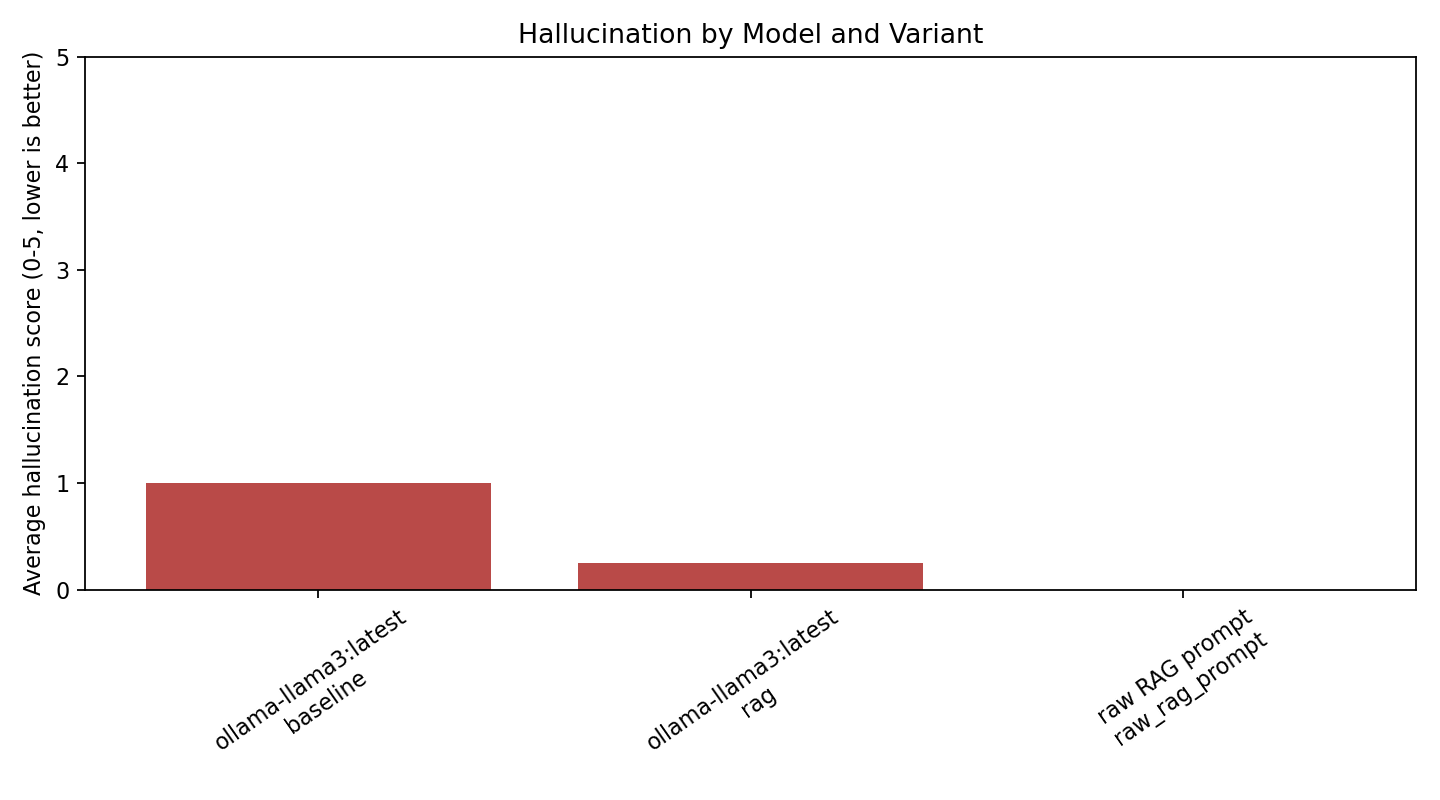
\includegraphics[width=\linewidth]{../evaluation/results/hallucination_by_model.png}
	\caption{\textbf{Hallucination rate comparison.} The bar chart illustrates the stark difference in hallucination tendencies;
	the RAG architecture significantly minimizes fabricated legal claims compared to the baseline model (lower is better).}
	\label{fig:hallucination}
\end{figure}

The most compelling finding of our implementation is the mitigation of legal hallucinations.
The baseline model registered a hallucination score of 1.00, demonstrating a propensity to confidently fabricate legal information when uncertain.
Imposing RAG dynamics violently curtailed this behavior, driving the hallucination score down to just 0.25 (as seen in Figure \ref{fig:hallucination}).

Furthermore, the baseline model proved entirely incapable of admitting missing knowledge, achieving a 0.00 Refusal Accuracy.
It forcefully attempted to answer every unanswerable question. In stark contrast, the RAG system successfully exhibited a 0.75 Refusal Accuracy,
accurately recognizing when the BM25 retrieval omitted relevant texts and safely declining to answer rather than providing dangerous misinformation.

Grounding marginally improved from 4.75 to 4.95 indicating the RAG model successfully utilized the parsed document metadata for formal citation.
A slight decline in raw correctness and completeness scores (3.85 from 4.15) constitutes an expected trade-off: the RAG model acts significantly more conservatively,
bound only to what it is provided, while the baseline model freely guesses broad (but unverified) concepts.

\subsubsection*{Retrieval Integrity}
Our retrieval module underwent isolated testing entirely independently of the LLM generation phase.
The BM25 Okapi index achieved an \textbf{87.5\% Hit Rate}, effectively recovering relevant laws for the vast majority of our queries at an average
context footprint of just 176.3 words.
However, it generated a \textbf{25.0\% False Evidence Rate} on unanswerable questions, meaning the system occasionally
fetched completely irrelevant statutes simply because they shared lexical token overlap with the query.
This indicates our architecture functions correctly at large but still demands improvement.

\subsubsection*{Analysis}

To better understand the numerical metrics, a qualitative review of the generated responses reveals clear behavioral patterns.
The RAG approach excels in scenarios requiring strict adherence to statutory limits and definitions.
For example, when queried about statutory severance pay (\textit{"Koliko znaša odpravnina?"}), the RAG system accurately grounds its answer in Article 108 of ZDR-1,
explaining the exact fractional logic (e.g., 1/5 of the base salary per year of employment).

Conversely, the baseline model frequently falls victim to plausible-sounding legal hallucinations.
When queried about specific rights or edge cases, the baseline model might authoritatively fabricate a rule---such as confidently claiming
"the employer must provide exactly 3 days of extra leave for moving" or misstating the mandatory notice period---and back it
up by citing a completely non-existent or irrelevant article number from the ZDR-1.
Our RAG implementation elegantly eliminates this behavior by forcing the model to either reliably cite the provided texts or admit ignorance.

Where the RAG system primarily fails is during "lexical mismatch" scenarios.
If a user poses a question using colloquial synonyms (e.g., asking about \textit{"bolniška"}
instead of the formal statutory term \textit{"začasna nezmožnost za delo"}),
the exact-match BM25 search might fail to retrieve the relevant passage.

Consequently, the LLM receives empty or irrelevant context and defaults to its prompt constraint, refusing to answer.
While this correctly avoids a hallucination, the resulting formal refusal is ultimately unhelpful to the user, portraying a brittle retrieval step.

\section*{Future Improvements}

While the current methodology establishes a robust baseline for legal question answering, we identify several areas for future enhancements.
At present, the retrieval component relies exclusively on exact lexical matching, meaning that legal documents can naturally be overlooked if the user phrases
their query using synonyms or colloquial terms that differ from the strict formal language of the statutes.

To address this limitation, we plan to explore the integration of dense vector embeddings and semantic search.
Incorporating models capable of deeply understanding the semantic meaning behind questions would allow the system to fetch relevant documents even when there
are no exact keyword overlaps, significantly increasing the recall and overall robustness of the retriever.
Furthermore, employing a hybrid retrieval approach---combining the precision of BM25 with the semantic recall of vector embeddings---paired
with a cross-encoder reranker, represents the most promising direction for elevating the assistant's factual accuracy in our next development phases.

%\subsection*{Equations}

%You can write equations inline, e.g. $\cos\pi=-1$, $E = m \cdot c^2$ and $\alpha$, or you can include them as separate objects. The Bayes’s rule is stated mathematically as:

%\begin{equation}
%	P(A|B) = \frac{P(B|A)P(A)}{P(B)},
%	\label{eq:bayes}
%\end{equation}

%where $A$ and $B$ are some events. You can also reference it -- the equation \ref{eq:bayes} describes the Bayes's rule.

%\subsection*{Lists}

%We can insert numbered and bullet lists:

% the [noitemsep] option makes the list more compact
%\begin{enumerate}[noitemsep]
%	\item First item in the list.
%	\item Second item in the list.
%	\item Third item in the list.
%\end{enumerate}

%\begin{itemize}[noitemsep]
%	\item First item in the list.
%	\item Second item in the list.
%	\item Third item in the list.
%\end{itemize}

%We can use the description environment to define or describe key terms and phrases.

%\begin{description}
%	\item[Word] What is a word?.
%	\item[Concept] What is a concept?
%	\item[Idea] What is an idea?
%\end{description}

%\subsection*{Figures}

%You can insert figures that span over the whole page, or over just a single column. The first one, \figurename~\ref{fig:column}, is an example of a figure that spans only across one of the two columns in the report.

%\begin{figure}[ht]\centering
%	\includegraphics[width=\linewidth]{single_column.pdf}
%	\caption{\textbf{A random visualization.} This is an example of a figure that spans only across one of the two columns.}
%	\label{fig:column}
%\end{figure}

%On the other hand, \figurename~\ref{fig:whole} is an example of a figure that spans across the whole page (across both columns) of the report.

% \begin{figure*} makes the figure take up the entire width of the page
%\begin{figure*}[ht]\centering
%	\includegraphics[width=\linewidth]{whole_page.pdf}
%	\caption{\textbf{Visualization of a Bayesian hierarchical model.} This is an example of a figure that spans the whole width of the report.}
%	\label{fig:whole}
%\end{figure*}


%\subsection*{Tables}

%Use the table environment to insert tables.

%\begin{table}[hbt]
%	\caption{Table of grades.}
%	\centering
%	\begin{tabular}{l l | r}
%		\toprule
%		\multicolumn{2}{c}{Name} \\
%		\cmidrule(r){1-2}
%		First name & Last Name & Grade \\
%		\midrule
%		John & Doe & $7.5$ \\
%		Jane & Doe & $10$ \\
%		Mike & Smith & $8$ \\
%		\bottomrule
%	\end{tabular}
%	\label{tab:label}
%\end{table}


%\subsection*{Code examples}

%You can also insert short code examples. You can specify them manually, or insert a whole file with code. Please avoid inserting long code snippets, advisors will have access to your repositories and can take a look at your code there. If necessary, you can use this technique to insert code (or pseudo code) of short algorithms that are crucial for the understanding of the manuscript.

%\lstset{language=Python}
%\lstset{caption={Insert code directly from a file.}}
%\lstset{label={lst:code_file}}
%\lstinputlisting[language=Python]{code/example.py}

%\lstset{language=R}
%\lstset{caption={Write the code you want to insert.}}
%\lstset{label={lst:code_direct}}
%\begin{lstlisting}
%import(dplyr)
%import(ggplot)

%ggplot(diamonds,
%	   aes(x=carat, y=price, color=cut)) +
%  geom_point() +
%  geom_smooth()
%\end{lstlisting}

%----------------------------------------------------------------------------------------
%	REFERENCE LIST
%----------------------------------------------------------------------------------------
\bibliographystyle{unsrt}
\bibliography{report}


\end{document}
